\label{chapter:approach}
In this work, we aim to build an approach able to (i) automatically test Android applications with modern state-of-art tools, (ii) automatically collect the arising errors (\ie stack traces), (iii) detect the unique errors (\ie the ones that derive from the same bug), (iv) link such stack traces with the user reviews that claim about the correspondent problems.           
We called this approach \textbf{BECLOMA} (\textbf{B}ug \textbf{E}xtractor, \textbf{C}lassifier and \textbf{L}inker \textbf{O}f \textbf{M}obile \textbf{A}pps).
Figure \ref{fig: becloma} depicts the main actions performed by this approach.
To give a clearer and more understandable explanation of how \toolname\ works, we will describe in the following Chapter its key features (see figure \ref{fig: becloma}). Such features represent the three main processes that \toolname\ sequentially performs.
\begin{enumerate}
\item the \textsc{Testing} part uses \monkey and \sapienz to test the APKs under test, reporting their testing results and extracting possible \textit{crashes} from the before generated test logs; 

\item the \textsc{Clustering} part investigates the similarity between the previous extracted crash logs, using different metrics and strategies, in order to collect them together and create a crash log \textit{bucket}, \ie a set of unique; 

\item the \textsc{Linking} part represents the core feature of \toolname. It preprocesses a set of given \textit{user reviews} as well as the set of the previously created crash logs, in order to preprocess them for the linking procedure. Afterwards, it investigates whether there exists a correlation between the stack traces and the user feedbacks, with the aim to link, if possible, the reviews with the crash logs. 
\end{enumerate}
\begin{figure}[tb]
\centering 
%	\vspace{-1.5mm} 
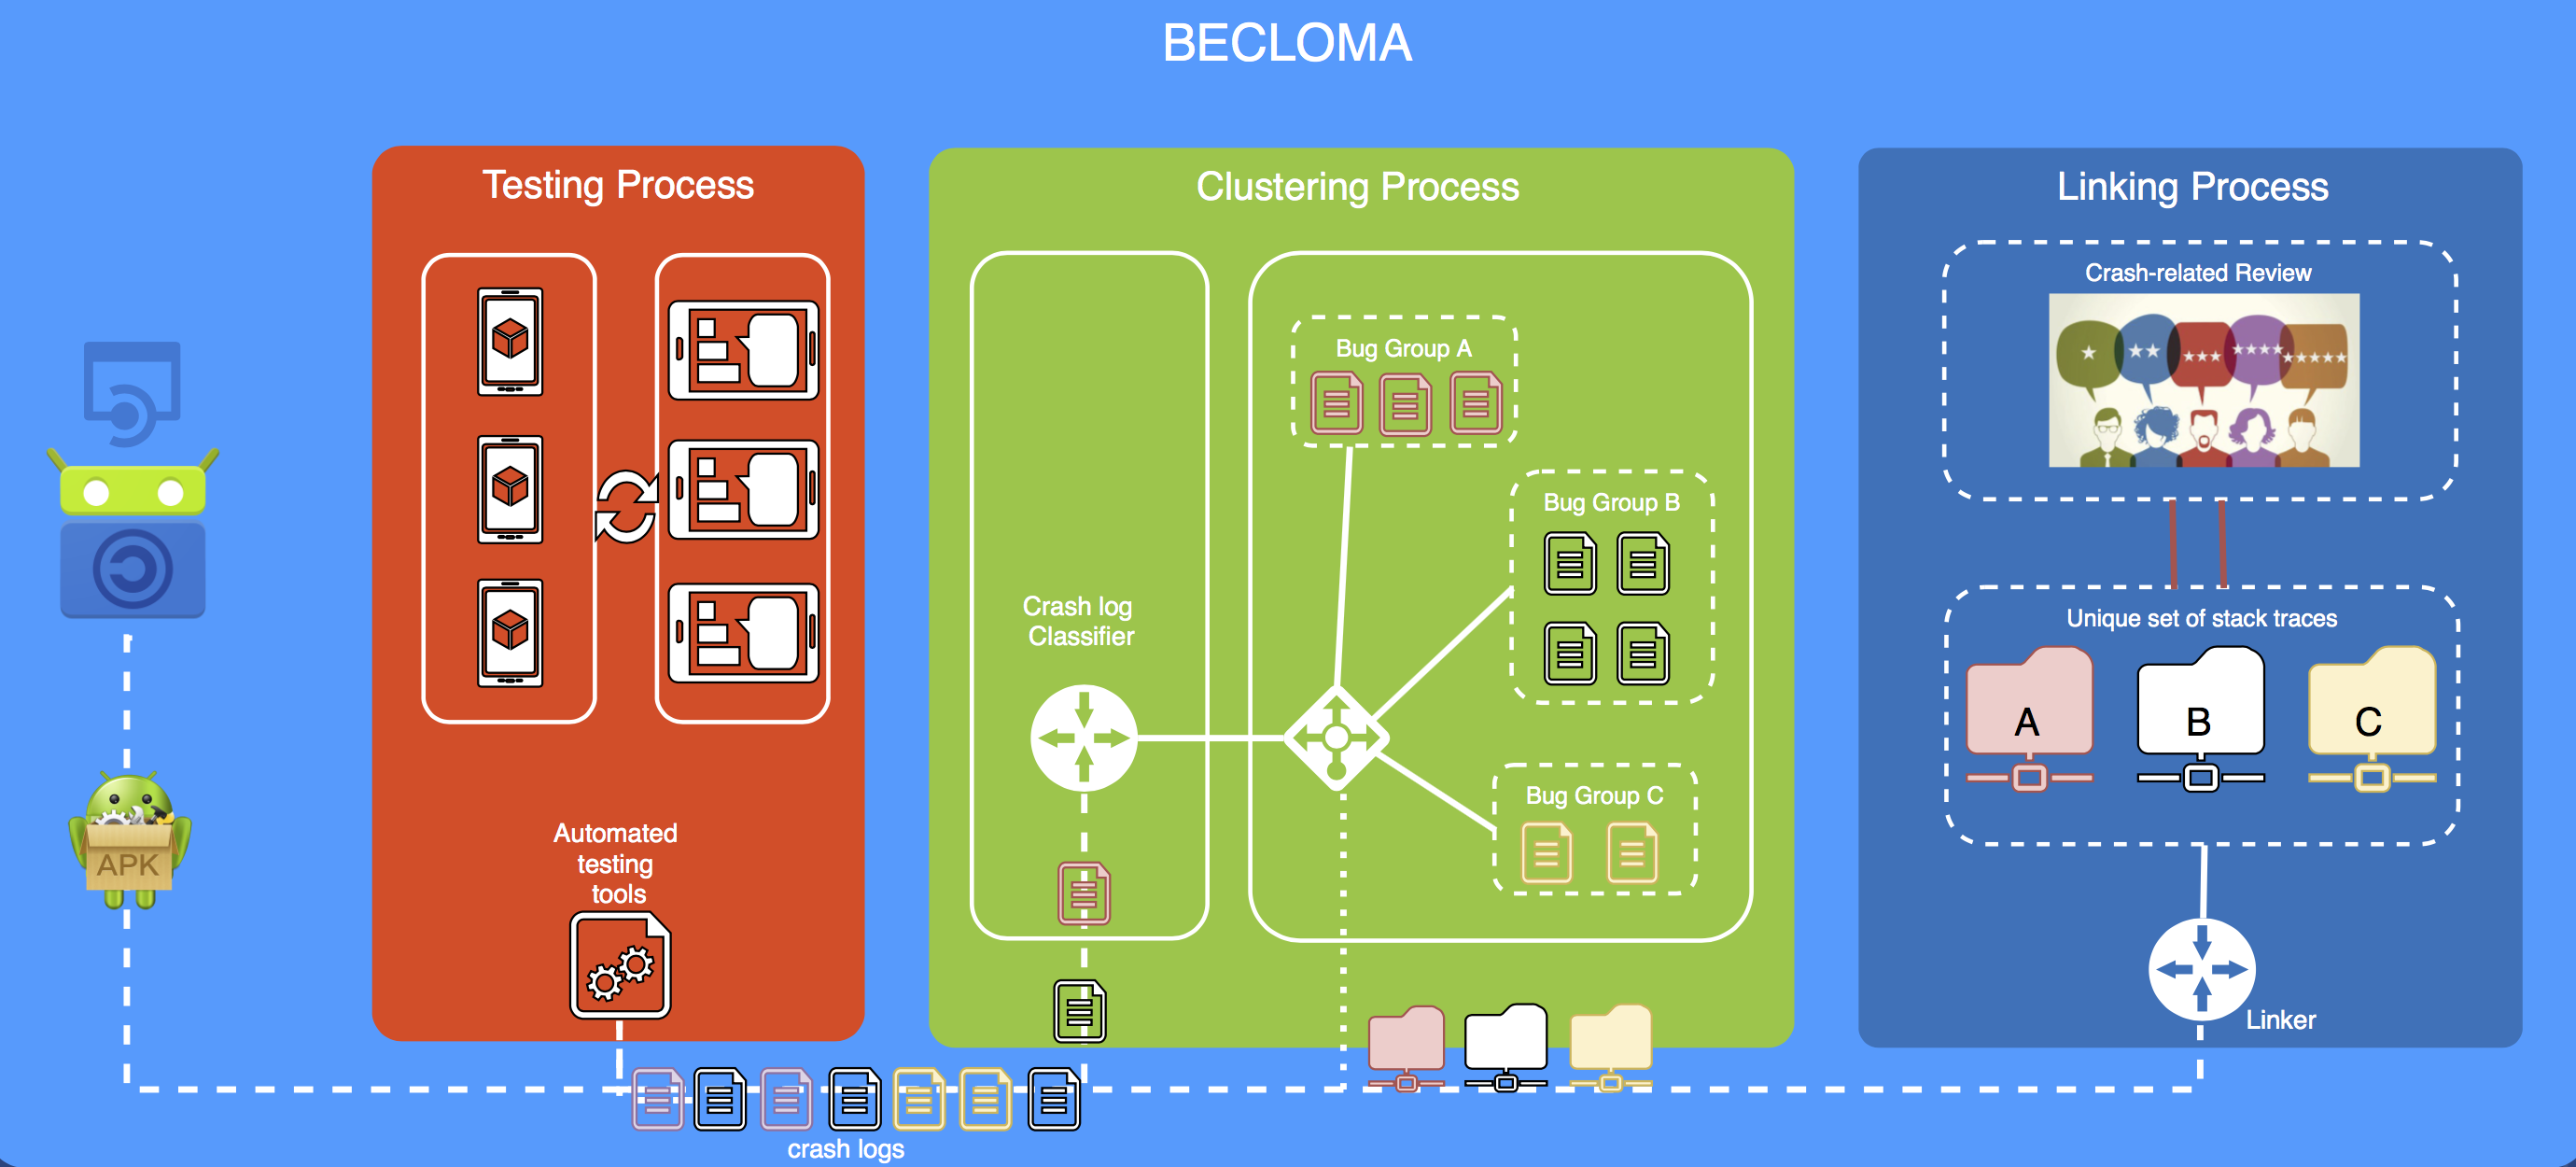
\includegraphics[width=\columnwidth]{diagrams/becloma_approach_img} 
\caption{\toolname\ approach}
\label{fig: becloma}
\end{figure}


\section{Testing and Traces Collection}
\label{approach:testing}
The first step in the overall approach basically relies on two of the most used Android testing tools, in order to exercise the SUT under tests and collect as many failures as possible. 
First of all, \toolname\ acts as crawler in order to download the set of desired APKs from the \textit{FDroid} API. 
Thus, it firstly reads a static structured file containing a set of android package names; then, it builds the necessary \textit{HTTP links} in order to download the corresponding APK files. 
Once the dataset has been built and some testing parameters have been specified, the testing session can be started. 
The set of parameters that must be specified are described in detail in Section \ref{usage: settings}.
The overall approach of \toolname\ consists in three testing cycles: 
\begin{enumerate}
\item 
The \textbf{single app} cycle concerning the testing of a single APK. It represents the time frame for which each APK in the dataset is tested. After that time frame, the approach starts with the testing of the next APK indicated in the dataset. 
\item The \textbf{dataset} cycle describing the time spent for testing the APKs within the dataset exactly one time for that currently cycle. 
\item The \textbf{session} cycle characterizing a testing session, \ie how many dataset cycles have to be performed. 
\end{enumerate}
Figure \ref{fig: testingapproach} shows the roles of these cycles in the testing approach, while figure \ref{fig: apkprocess} illustrates the process in detail behind the \textit{single app cycle}. 
First, during this cycle the APK is systematically \textit{tested} according to its specifications and testing parameters. 
Once the test is finished, the \textit{reporting} phase starts. 
This step consists of saving the generated reports in a given directory. 
Once the logs have been stored, they are ready to be \textit{investigated}. This means, that the reports are parsed with the intention to find eventually crashes inside them. 
Afterwards, if a crash occurred, its part relative to the stack trace from the whole corpus of the log is \textit{extracted}. At the end, this information is saved into a specific directory aiming at collecting all the arose failures.

\begin{figure}[tb]
\centering 
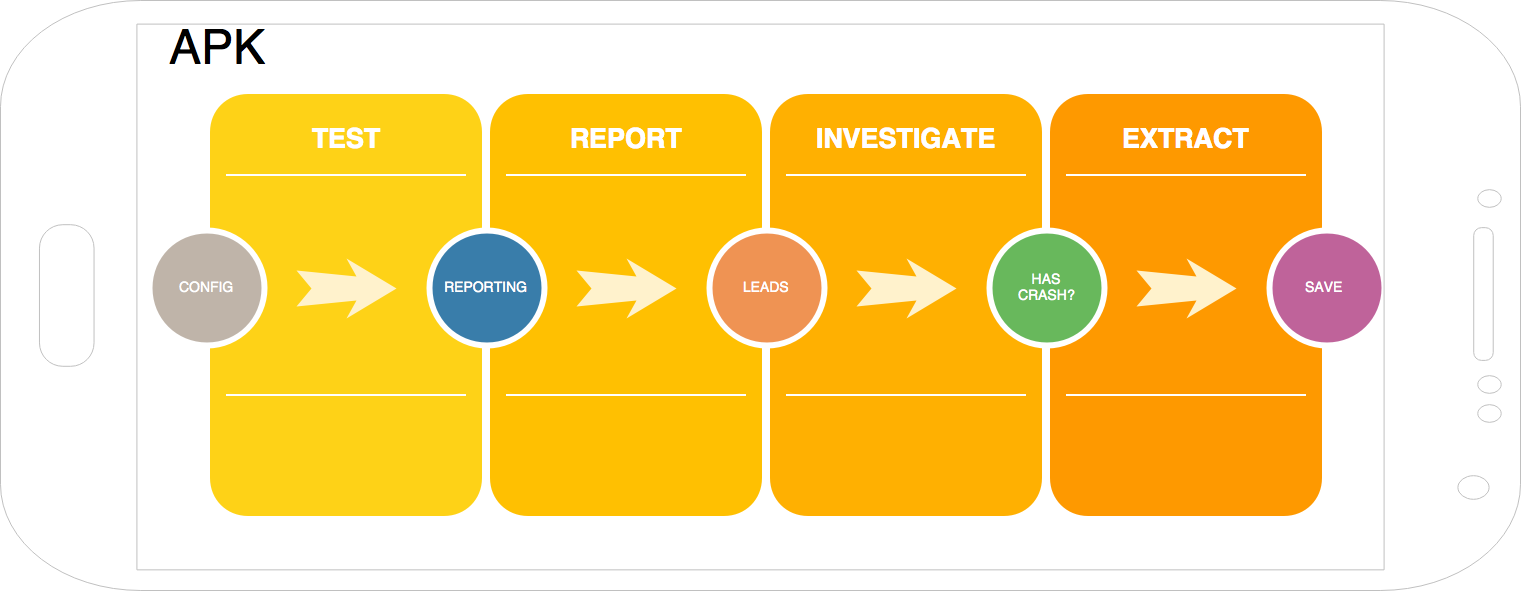
\includegraphics[width=12.5cm,height=5cm]{imgs/apkprocess} 
\caption{Approach performed by \toolname\ for testing a single Android app}
\label{fig: apkprocess}
\end{figure}

\begin{figure}[tb]
\centering 
%	\vspace{-1.5mm} 
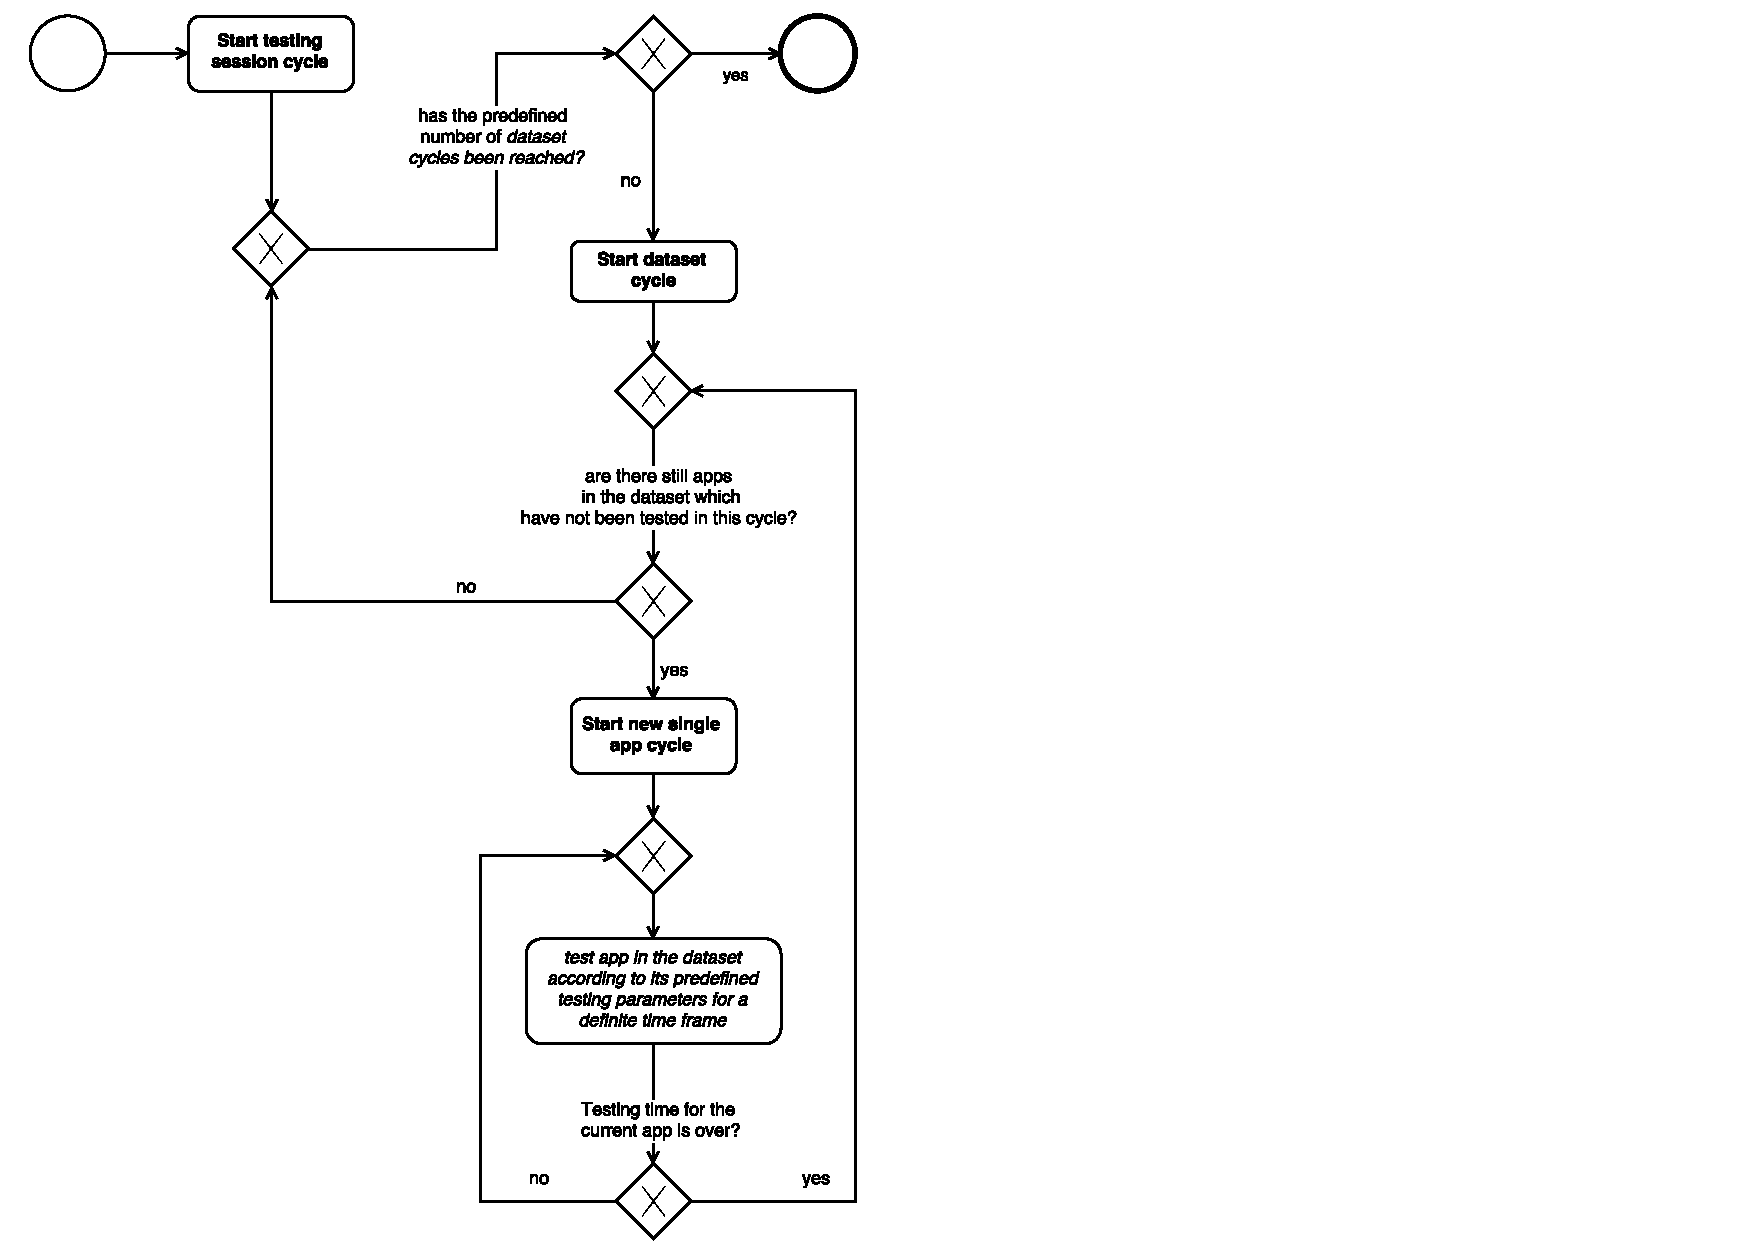
\includegraphics[width=13cm,height=17cm]{diagrams/testingapproach} 
\caption{Testing cycles characterizing the testing approach}
\label{fig: testingapproach}
\end{figure}

%that contain the stack traces of the runtime exceptions detected by the tools together with the sequence of the UI and/or system events that led to the failures [6].


\clearpage
\section{Clustering of the Collected Traces}
\label{approach:clustering}
As we said before, at the end of the testing phase all the stack traces that have been generated are stored in a specific directory. However, it is worth noticing that with a high change, most part of such failures would refer to the same bug. %(in other words, the traces are duplicates). 
\LUCAS{si capisce ora cosa sono gli unique crashes?}
To make our explanation better understandable, we introduce a new term we call \textit{unique crashes}. 
In this sense, a set of unique crashes indicates a group of duplicates in the cluster which belong to the same bug. In fact, each crash in that cluster is considered to be interchangeable.

 
Indeed, in order to identify these unique crashes, the second step of our approach performs an automatic clustering of the overall bunch of logs. Ideally, at the end of such phase, each cluster should contain logs that refers to exactly the same bug.
For this task, we rely on classic Information Retrieval (IR) techniques, collecting features about the logs and comparing them using the \textit{cosine similarity} metric.
Figure \ref{fig: clustering} shows the overall process for this task. 
\begin{figure}[tb]
\centering 
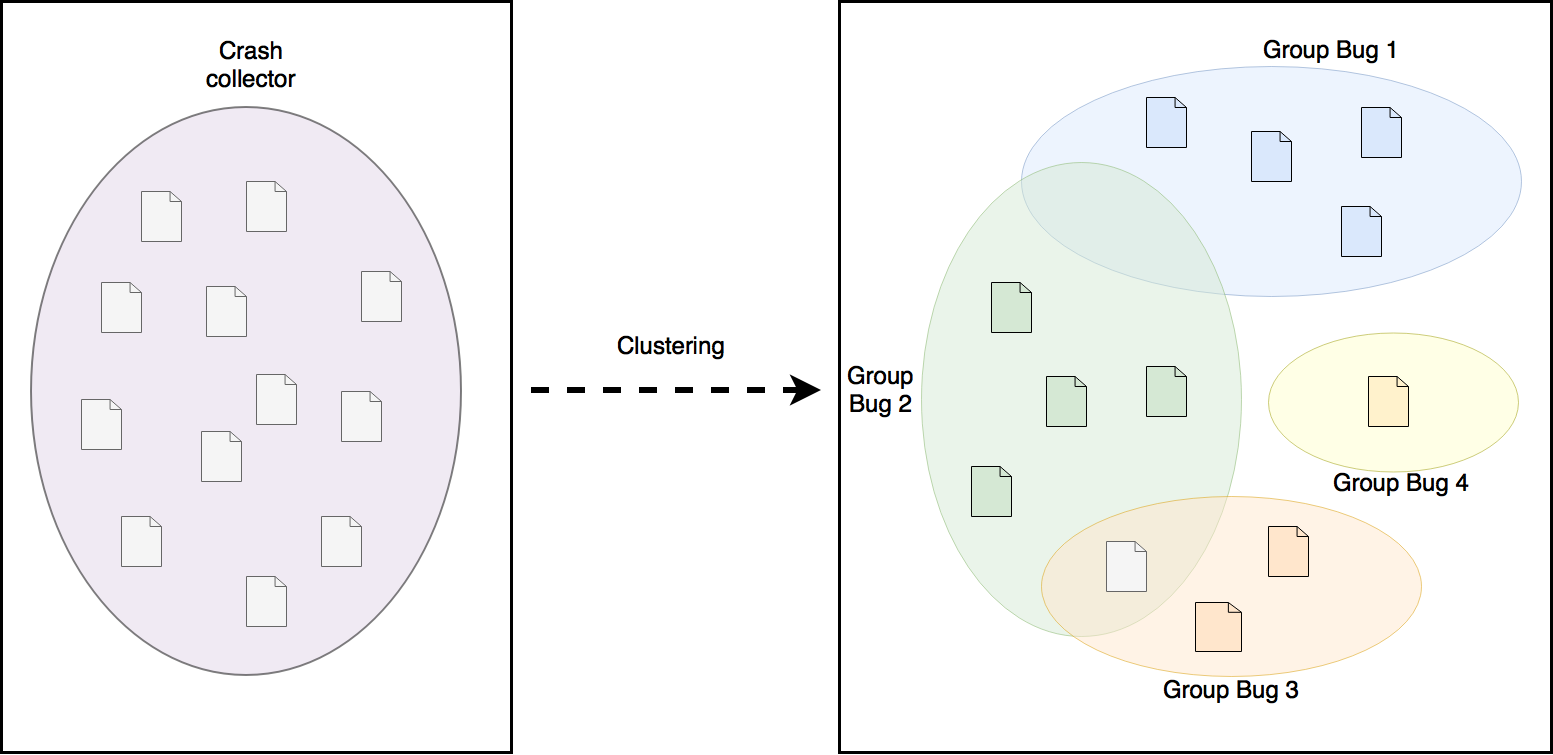
\includegraphics[width=\columnwidth]{imgs/clusteringidea} 
\caption{The idea behind the clustering process}
\label{fig: clustering}
\end{figure}
As said before, some track traces may be overlapping \ie refers to the same bug of be even duplicates. 
Despite the trigger method, \ie the method that raised to the exception, may be the same, there may be different sequences of function calls in the stack trace, the more the analysis goes deep. 
However, they are hardly detectable and is difficult to affirm that two stack traces which have the same trigger method refer to different bugs. 
Therefore, some reports may belong to two different bug groups in the bucket. 
In order to understand better the clustering approach, a clarification of how a crash log is structured must be done. 
For this purpose, the real structure of a crash report is illustrated in Listing~\ref{lst: ringdroid}. 
\begin{lstlisting}[caption=Structure of a crash log, basicstyle=\fontsize{6}{8}\ttfamily,label={lst: ringdroid}]
// CRASH: com.ringdroid (pid 6207)
// Short Msg: android.database.StaleDataException
// Long Msg: android.database.StaleDataException: Attempted to access a cursor after it has been closed.
// android.database.StaleDataException: Attempted to access a cursor after it has been closed.
// 	at android.database.BulkCursorToCursorAdaptor.throwIfCursorIsClosed(BulkCursorToCursorAdaptor.java:64)
// 	at android.database.BulkCursorToCursorAdaptor.getCount(BulkCursorToCursorAdaptor.java:70)
...
\end{lstlisting}
A crash log is usually structured as follows: 
\begin{itemize}
\item \textit{Line 1} represents the top of the crash log, where the concerned package name is made explicit;
\item \textit{Line 2} tells in few words the cause of the exception; 
\item \textit{Line 3} complements the cause of the exception giving a long explanation about the exception itself;
\item \textit{Line 4} represents the first line of the stack trace and contains the name and the generic cause of the exception. 
From this point, all the function calls underlying are part of the stack trace;
\item \textit{Line 5} is considered the exact reason for the exception, \ie the trigger method within the source code that caused the crash;
\item From \textit{line 6} moving gradually down until the end of the stack trace, there are other nested function calls which contain additional information about the cause of the exception. Usually, the most important ones for identifying the cause are in the first few lines. 
\end{itemize}
%\GIO{Specify that we used a search based approach to identify the correct threshold to choose whether two logs are the same or not}
In order to state whether two crash reports refer to the same bug or not, we used a search based approach to identify the correct threshold. 
Indeed, we built an \textit{Oracle} which is in charge of comparing two crash logs and is able to answer the following question: \textit{Do they refer to the same bug?}. 
For its answers it makes use of a similarity tolerance, which has been adapted on the base of our experimental results. 
In fact, we manually created the bucket of unique crash logs and consequently adapted the threshold in the oracle in order to enable it to rightly answer its questions and so reproduce the same bucket. 

\paragraph{Preprocessing.}
The first step of the clustering approach consists in \textit{preprocessing} the crash reports in order to prepare them to be compared to each other.
\LUCAS{Seba: just explain why it is important to perform this preprocessing step}
The preprocessing step is fundamental to be performed since (i) it removes possible noise from the logs (remove unless symbols or numbers), (ii) standardizes them making their contents consistent to each other and (iii) parses and converts them identifying different key elements. 
To perform such phase, the approach follows a grammar-based tokenization technique implemented in the well-know \textbf{Apache Lucene} \cite{lucene} library.  
%Indeed, all words contained in the crash reports are preprocessed using \textbf{Apache}. 
In this respect, we collected all words contained in the crash reports and preprocessed them using a Lucene tokenizer, called \textit{Standard Tokenizer} \cite{lucenestandardanalyser}. 
%\GIO{Do not use too often ''the approach consists''! You can use 'it' or 'we'}
This tokenizer simply splits the word fields into lexical units using punctuation and whitespaces as split points. In addition, it removes unnecessary symbols (\eg \texttt{"//"}).
\toolname\ extends the Lucene tokenizer to a further CamelCase regular expression.
This because it is a worldwide convention that developers use CamelCase notation for writing programming words such as names of classes, names of functions or names of variables.
Since most of the words included in the crash logs are programming language keywords, \toolname\ complements such StandardTokenizer, so that CamelCase text fields can be also split at the upper-case letters into separate words. 

\paragraph{TF-IDF.} 
Once all words inside the crash logs have been tokenized, we relied on some well know Information Retrieval techniques in order to link together the duplicated crashes.
As features for such process, we relied on the computation of the tf-idf \textit{(term frequency inverse document frequency)} values on the collected stack traces. 
In this direction, \toolname\ computes tf-idf numerical statistics in order to find the relevance of a word in a collection of documents (in our case, the crash logs). 
Tf-idf is a well-know term-weighting scheme and usually is used in Information Retrieval or text mining \cite{tfidf}. %Indeed, tf-idf is a way to measure the relevance, the weight of a term compared to its document or its entire document collection (in our case, the crash logs). 
The importance of a term is given by the number of times it occurs in a particular document, inversely proportional to its appearance in the entire documents collection \cite{campbell}. 
%\GIO{The tfidf is not an algorithm. That's a statistics that measure the importance of a word in a set on document. Slightly modify this section changing a bit the terminology}
Generally, a tf-idf scheme consists of three main components \cite{tfidfsimilarity}: 
\begin{itemize}
\item \textbf{TF (Term Frequency)}, \ie how many times a term appears in the currently scored document, where repeated terms indicate the topic of the document; A high \textit{tf} means that the word in question has a high relevance for the document. The following simplified equation \cite{tfidf} describes a formula for calculating it:
\begin{align*}
tf_{x,y} = \frac{n_{x,y}}{\mid d_{y} \mid}
\end{align*}
where $n_{x,y}$ represents the number of occurrences of the term $t_x$ in the document $d_{y}$, while $\mid d_{y} \mid$ represents the number of words inside the document $d_{y}$.

\item \textbf{IDF (Inverse Document Frequency)}, \ie the inverse of the document frequency, that represents the number of document in which the term appears. 
If the same term appears in fewer documents, \textit{idf} shows a high value, whereas if a term is very common it returns a low value. 
The equation \cite{tfidf} below describes a simplified version of the inverse document frequency formula: 
\begin{align*}
idf_{x} = \frac{\mid D \mid}{\mid \{d: t_{i} \in d\} \mid}
\end{align*}
where $\mid D \mid$ is the number of documents in the collection, while $\mid \{d: t_{i} \in d\} \mid$ represents the number of documents which contains the term $t_i$

\item TF-IDF, \ie the product of the two above terms. If it has a high value means that the currently scored term has a high relevance, otherwise if it returns a low value, the term has little relevance.
\begin{align*}
tfidf_{x,y} = tf_{x,y}*idf_{x}
\end{align*}

\end{itemize}
The \textit{idf} metric actually measures how important a term is. 
This because a term which appears very often in a single document will have a high \textit{tf} score but if this term rarely occurs in the other ones it will also have have a high \textit{idf} score and so a low tf-idf value. 
This would imply that it shall not have a high relevance. 
Otherwise, if a word occurs very often both in a single document and in the entire collection it has a high \textit{tf} score and a low \textit{idf} value, which results in a high tf-idf score. \\
At the end of this phase, \toolname\ has created for each crash log its correspondent vector space model, \ie a weighted vector term, where each term indicates a new dimension in the vector and is associated with its correspondent tf-idf value. 


\paragraph{Cosine Similarity.}
\label{sec:cosine_similarity}
To state whether two crash reports refer to the same bug, the approach computes cosine similarity between their previously created vectors space model. 
The cosine similarity is just a measure of similarity between two vectors \cite{cosine} (in our case, two normalized weighted vectors consisting of their tf-idf scores).
Usually, the resulting similarity ranges from -1 to 1, but in the case of Information Retrieval, since the frequency of the terms are always positive, the returned values range from 0 to 1, where 0 indicates that two documents are completely decorrelated, while 1 means that the words contained inside them are exactly the same.  
The equation describing the cosine similarity between two vectors is as follows: 
\begin{align*}
cosine\:similarity = \cos({\theta}) = \frac{A\cdot{B}}{||A||\:||B||}
\end{align*}
where, in our case $A$ and $B$ are two normalized weighted term vectors consisting of tf-idf values. 
With the term "normalized" is understood that when two weighted vectors are used to compute cosine similarity among them, for each time a word is contained within a vector but not in the other, that term is inserted into the vector that does not contain it by associating a tf-idf score of 0. Furthermore, in doing so the two vectors will have the same length by making the computation of their dot product possible. 



\section{Linking approach}
\label{approach:linking}
\label{par: infusa}
To study the correlation between user reviews and the outcomes of automated testing tools, \toolname\ assumes that the set of users feedback have been already classified in according to a defined taxonomy and preprocessed.
In order to classify the users feedback according to a given taxonomy (and ad oc preprocessed) we relied on an approach implemented by Palomba \etal \cite{Palomba2017}. 
In this approach, they proposed some machine learning techniques for automatically classifying a set of user reviews according to a defined taxonomy. 
%\GIO{This is not super correct. In order to classify the user feedback according to a given taxonomy (and ad hoc preprocessed) we relied on the implementation done by Fabio Palomba and Adelina Ciurumelea in the paper that is also in the references. Use such paper as a reference when citing the such approach. The INFUSE-TA tools uses this approach in order to classify the reviews to link them to the logs}.
Furthermore, it performs a systematic Information Retrieval (IR) preprocessing \cite{BaezaYates:1999} on both the user reviews and \textit{augmented} stack traces aimed at (i) correcting mistakes, (ii) expanding contractions (e.g., \textit{can’t} is replaced with \textit{can not}), (iii) filtering nouns and verbs, (iv) removing common words or programming language keywords, and (v) stemming words (e.g., \textit{aiming} is replaced with \textit{aim}). \\
The text below depicts an example of Information Retrieval preprocessing applied on a user feedback: 
\smallbreak
\emph{\small``Crashes on Messages I would give this 5 stars but it crashes every time I try to access my messages in the app. I have removed and reinstalled the app  signed in and out  even reformatted my phone. But it still crashes when I click Messages  every time without fail.''}. 
\smallbreak
\hspace{-1.5em}Following, the review is preprocessed applying the techniques described above:
\smallbreak
\emph{\small``crash messag i would give 5 star crash everi time i tri access messag app i remov reinstal app  sign  even reformat phone but still crash i click messag  everi time without fail''}. 
\smallbreak

%\hspace{-1.5em}In this direction, another experimental called \textbf{INFUSE-TA} (\textbf{IN}tegrator o\textbf{F} \textbf{US}er \textbf{FE}edback while Testing \textbf{A}pps) developed by a team at the Software Evolution and Architecture Lab, uses the approach proposed by Palomba \etal in order to classify the reviews and link them to the crash reports. 

\paragraph{Linking between Crash Logs and Reviews}
The last step of the approach consists of linking the information from the stack traces contained in the reports to the relevant user reviews. 
However, linking the two sources of information is not at all obvious.
This because they come from different worlds: user reviews contain natural human language which describe the overall scenario that led to a failure \cite{mernik}, while the stack traces contain technical information about the exceptions raised during the execution of a certain test case. 
To account for this aspect, the approach first removes all information that creates noise in the collected stack traces, only the name and cause of the raised exceptions are selected, \ie the first line of the stack trace (in the example \ref{lst: ringdroid} the \textit{line 4}). 
The choice of considering only some specific parts of the stack traces was driven by experimental results. 
These results illustrated how the linking accuracy was influenced by the presence/absence of this information. 
After cleaning the reports, the remaining text is \textit{augmented} with the source code methods included in the stack trace. 
This concretely means that each method extracted from the stack trace gets compared with all methods included in the source code. 
If a correlation among them exist, the stack trace is \textit{augmented} with the body and the set of words related to the that method. 
This step extends the information from the reports with contextual information from the source code, possibly providing additional information useful for the linking process. Also in this case, the choice was not random but driven by the experimental results.
Afterwards, the approach performs the systematic Information Retrieval (IR) preprocessing \cite{BaezaYates:1999} used by the approach implemented by \textit{Palomba} \textit{et al}. 
Finally, the resulting documents are linked using the asymmetric Dice similarity coefficient \cite{BaezaYates:1999}, which is defined as
follows: 
\begin{align*}
Dice (review_j, crash_i) = \frac{|W_{review_j} \cap W_{crash_i}|}{\textit{min}(|W_{review_j}|, |W_{crash_i}|)}
\end{align*}
where $W_{review_j}$ represents the set of words composing a user review $j$, $W_{crash_i}$ is the set of words contained in an augmented stack trace $i$ and the $min$ function normalizes the Dice score with respect to the number of words contained in the shortest document between $j$ and $i$. 
The asymmetric Dice similarity returns values between [0,1]. 
In my thesis, pairs of documents having a Dice score higher than \textbf{0.5} were considered as linked by the approach.






